\begin{mainquestion}{symmetricalcircuits}{Symmetrical Circuits}

\questionpoints
Determine the equivalent resistance $R$ measured between the two terminals of the flattened (two-dimensional) hexagon, if all resistors are $1.0~\mathrm{k}\Omega$.

\begin{center}
    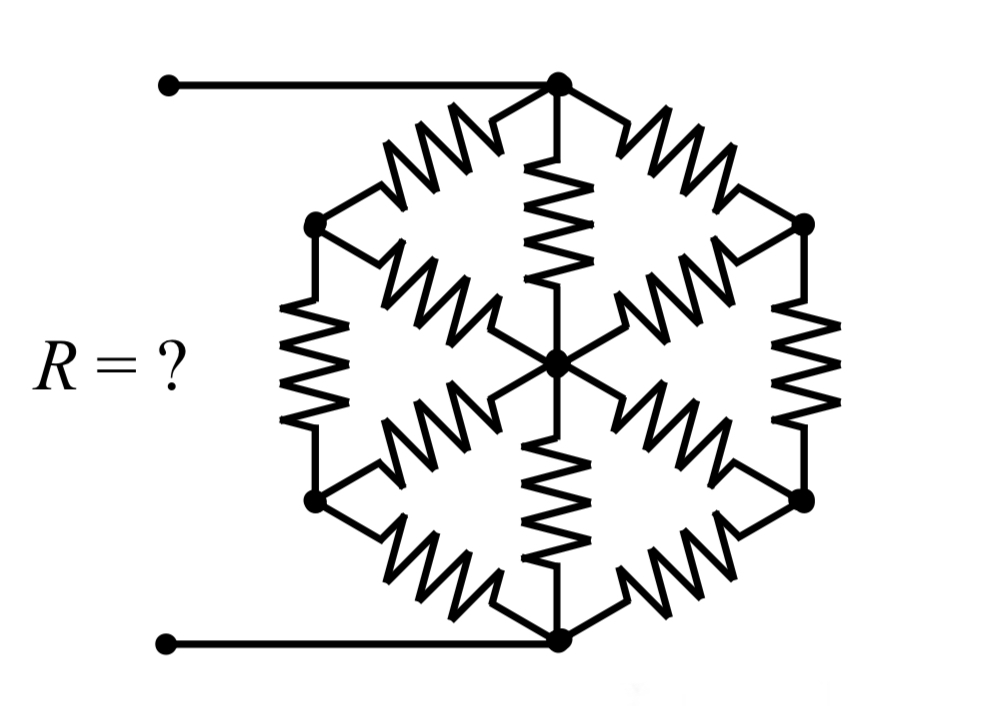
\includegraphics[width=0.6\textwidth]{question_2.jpeg}
\end{center}

\begin{answer}
\begin{center}
\begin{circuitikz}[scale=1]
    % Terminals
    \draw (0,2) node[left]{$A$} -- (1,2);
    \draw (0,0) node[left]{$B$} -- (1,0);

    % Left branch RL
    \draw (1,2) -- (2,2)
          to[R=$R_L$] (2,0)
          -- (1,0);

    % Middle branch RM
    \draw (3,2) -- (3,2)
          to[R=$R_M$] (3,0);

    % Right branch RR
    \draw (5,2) -- (4,2)
          to[R=$R_R$] (4,0)
          -- (5,0);

    % Top and bottom rails
    \draw (1,2) -- (5,2);
    \draw (1,0) -- (5,0);
\end{circuitikz}
\end{center}

By symmetry, the left and right halves of the network are identical, so we denote their equivalent resistances by $R_L$ and $R_R$, with
\[
R_L = R_R.
\]
The central vertical branch is denoted by $R_M$.

\medskip
\noindent
\textbf{Step 1: Reduce the middle branch.}

The middle branch consists of two resistors of value $1.5~\text{k}\Omega$ in series, so
\[
R_M = 1.0 + 1.0 = 2~\text{k}\Omega.
\]

\medskip
\noindent
\textbf{Step 2: Reduce the left (and right) branch.}

In the left branch, the top and bottom resistors are each $1~\text{k}\Omega$ in series with a parallel combination of
\[
\frac{1}{2~\text{k}\Omega} + \frac{1}{1~\text{k}\Omega}.
\]
Thus,
\[
R_L = 2 + \frac{1}{\dfrac{1}{2} + 1}
= 2 + \frac{1}{\dfrac{3}{2}}
= 2 + \frac{2}{3}
= \frac{8}{3}~\text{k}\Omega.
\]
By symmetry,
\[
R_R = \frac{8}{3}~\text{k}\Omega.
\]

\medskip
\noindent
\textbf{Step 3: Combine the three branches in parallel.}

The total resistance is the parallel combination of $R_L$, $R_M$, and $R_R$:
\[
\frac{1}{R_T}
= \frac{1}{R_L} + \frac{1}{R_M} + \frac{1}{R_R}
= \frac{1}{\frac{8}{3}} + \frac{1}{2} + \frac{1}{\frac{8}{3}}.
\]

\medskip
\noindent
\textbf{Step 4: Evaluate.}

\[
\frac{1}{R_T}
= \frac{3}{8} + \frac{1}{2} + \frac{3}{8}
= \frac{3}{8} + \frac{4}{8} + \frac{3}{8}
= \frac{10}{8}.
\]

Therefore,
\[
R_T = \frac{8}{10} = 0.8~\text{k}\Omega.
\]

\[
\boxed{R_T = 0.8~\text{k}\Omega.}
\]
\end{answer}

\end{mainquestion}
